% BTP final report -- ISAC-NET
% Compile: pdflatex main && pdflatex main   (or latexmk -pdf main)
% Works on Overleaf as-is (upload this folder with figures/).
\documentclass[11pt,a4paper]{article}

\usepackage[a4paper,margin=1in]{geometry}
\usepackage[T1]{fontenc}
\usepackage{lmodern}
\usepackage{amsmath,amssymb,bm}
\usepackage{graphicx}
\usepackage{booktabs}
\usepackage{array}
\usepackage{tabularx}
\usepackage{caption}
\usepackage{enumitem}
\usepackage{float}
\usepackage[colorlinks=true, citecolor=blue, linkcolor=black, urlcolor=black]{hyperref}
\usepackage{xcolor}
\makeatletter
\renewcommand{\@cite}[2]{\textcolor{blue}{[{#1\if@tempswa , #2\fi}]}}
\makeatother
\pdfstringdefDisableCommands{\def\ensuremath#1{#1}}

\graphicspath{{figures/}}
\captionsetup{font=small,labelfont=bf}
\setlist{itemsep=2pt,topsep=4pt}
\renewcommand{\arraystretch}{1.15}

% ---------- personal details: EDIT THESE ----------
\newcommand{\studentname}{Kushal Dornahalli}       % check spelling
\newcommand{\rollno}{230102052}                      % e.g. 230 1xx xxx
\newcommand{\department}{Department of Electronics and Electrical Engineering} % check
\newcommand{\supervisor}{Prof. Manoj BR}
\newcommand{\reportdate}{November 2026}
% --------------------------------------------------

\newcommand{\sci}[2]{\ensuremath{#1\times10^{#2}}}
\newcommand{\BH}{\mathbf{H}}
\newcommand{\BX}{\mathbf{X}}
\newcommand{\BY}{\mathbf{Y}}
\newcommand{\BZ}{\mathbf{Z}}

\begin{document}

% ================= TITLE BLOCK (same layout as previous BTP reports) =================
\begin{center}
  {\Large Clutter-Robust Deep-Unfolded Receivers for Integrated\\[2pt] Passive Sensing and Communication\par}
  \vspace{10pt}
  {\large \studentname\ (\rollno)\par}
  \vspace{4pt}
  \department\par
  Indian Institute of Technology Guwahati\par
  \vspace{4pt}
  B.Tech Project (7th semester) \quad Supervisor: \supervisor\par
  \vspace{4pt}
  \reportdate
\end{center}

\vspace{6pt}
\begin{abstract}
\noindent In integrated passive sensing and communication (IPSAC), a single receiver must decode the transmitted data and estimate the range and velocity of targets from the same received signal, without knowing the data in advance. ISAC-NET~\cite{isacnet} solves this with an iterative algorithm that alternates symbol detection, passive sensing and channel reconstruction, and unfolds it into a network whose 25 step-size parameters are learned from data.

This project reproduces ISAC-NET end to end at the paper's full simulation size (256 OFDM symbols $\times$ 1024 subcarriers, $8\times 8$ antennas, 3 targets) in Python and PyTorch, together with the LS, D-AMP and 2D-DFT baselines, under the paper's own simulation setup. Learning the parameters lowers the bit error rate (BER) by 4-11$\times$ at 15--25~dB and the velocity NMSE by about 5$\times$ at 20~dB compared with the hand-set algorithm.

Since the paper's channel has no clutter, we add distributed clutter scatterers to the channel model as a first extension. Communication stays robust (ISAC-NET keeps a 3-6$\times$ BER gain), but sensing breaks down with as few as five scatterers, because the peak extraction reports clutter as targets, and retraining the step sizes on clutter does not fix it. This motivates the proposed research direction: a clutter-robust ISAC-NET with a learned clutter-suppression stage before sensing.
\end{abstract}

\vspace{8pt}
{\setcounter{tocdepth}{1}\small\tableofcontents}
\newpage

% =====================================================================
\section{Introduction}
Integrated sensing and communication (ISAC) lets one radio system share spectrum and hardware between data transmission and target sensing, and is a candidate feature of 6G networks~\cite{isacnet,zhang2022}. In \emph{active} (monostatic) sensing the receiver sits next to the transmitter and knows the transmitted waveform. In \emph{passive} (bistatic) sensing the sensing receiver is a communication receiver at another site. It avoids full-duplex self-interference, but it does not know the data symbols, so it must decode them before it can use them as a sensing reference.

Sensing from the pilots alone wastes most of the frame, since pilots fill only 1 of every 14 OFDM symbols. Sensing from the data needs correctly decoded symbols, and decoding errors corrupt the sensing estimate, which in turn corrupts the channel used for decoding. ISAC-NET~\cite{isacnet} handles this loop jointly. Its iterative algorithm (Alg.~3 of~\cite{isacnet}) alternates improved D-AMP detection, 2D-DFT range--Doppler sensing on the detected symbols, and channel reconstruction from the sensed targets. Because the result depends on 5 hand-set parameters per iteration, the authors unfold the iterations into network layers and learn those parameters, a form of model-driven deep learning known as deep unfolding~\cite{oampnet}.

\subsection{Objectives}
Aim of this project was to reproduce ISAC-NET faithfully enough to test its claims, finding where its approach is weak and extending it to introduce clutter in the channel.

\subsection{Contributions}
\begin{enumerate}
  \item An open Python/PyTorch implementation of the full system model, three baselines, Alg.~3 and ISAC-NET at the paper's Table~III size, with unit tests (\url{https://github.com/Kushal2oo4/isac-net}).
  \item A list of points where the paper is ambiguous or inconsistent, the choice made for each, and an explanation of why our figures differ from the published ones.
  \item A reproduction of the paper's main claim under its own setup: learning lowers BER by 4--11$\times$ compared with the hand-set algorithm.
  % \item Findings beyond the paper: the learned parameters transfer only partly to unseen target layouts, and the last layer partly undoes the convergence of the earlier ones.
  \item A first extension: clutter scatterers in the channel model, showing that ISAC-NET's sensing fails under clutter, which defines the research direction for future work.
\end{enumerate}

Section~\ref{sec:background} reviews background, Section~\ref{sec:model} gives the system model, Section~\ref{sec:algos} the algorithms and Section~\ref{sec:impl} the implementation and setup. Section~\ref{sec:results} presents the results, Section~\ref{sec:future} the proposed future work, and Section~\ref{sec:conclusion} concludes.

% =====================================================================
\section{Background}\label{sec:background}
\subsection{OFDM radar sensing}
With OFDM, the radar channel can be read directly from the data: dividing each received resource element by the transmitted symbol removes the modulation, leaving a matrix whose phase rotates with delay across subcarriers and with Doppler across symbols. An inverse DFT over subcarriers and a DFT over symbols then give a range-velocity map, whose peaks are the targets~\cite{sturm2011}. This works only when the transmitted symbols are known, which is why passive sensing depends on correct detection.

\subsection{Deep unfolding}
An iterative algorithm with a fixed number of iterations can be written as a feed-forward network, one layer per iteration. Its hand-set parameters (step sizes, damping factors, thresholds) become trainable weights, while the structure of the algorithm is kept. The result needs far fewer parameters and training samples than a black-box network and stays interpretable. OAMP-Net2~\cite{oampnet} applies this to MIMO detection and is one of the baselines in~\cite{isacnet}.

\subsection{ISAC-NET}
ISAC-NET~\cite{isacnet} combines the two: it unfolds an iterative receiver that detects symbols, senses targets from the detected symbols, and rebuilds the channel from the targets. It reports BER close to OAMP-Net2 and better than a model-free network (TPG), with range and velocity NMSE close to the Cram\'er--Rao bound at high SNR. Its learned parameters are trained offline and stored separately for each SNR.

% =====================================================================
\section{System Model}\label{sec:model}
A base station with $N_t$ antennas sends an OFDM frame of $M$ symbols $\times$ $N$ subcarriers. A receiver with $N_r$ antennas at another site decodes the data and senses $L_p$ point targets from their echoes, following~\cite[Sec.~II]{isacnet}.

\subsection{Transmitted frame}
The same symbol $x(m,n)$ is sent on every transmit antenna, so the transmit vector is $\mathbf{x}(m,n)=[x(m,n),\dots,x(m,n)]^T$. One of every 14 OFDM symbols is a known QPSK pilot; the rest carry 16-QAM data.

\subsection{Channel}
Each target reflects the signal once. Path $l$ has length $r_l=r_{1,l}+r_{2,l}$ (transmitter to target plus target to receiver), delay $\tau_l=r_l/c$ and Doppler shift $f_{d,l}=v_l f_c/c$. Its channel at symbol $m$ and subcarrier $n$ is
\begin{equation}
  \tilde{\BH}_l(m,n)=\sqrt{F_l}\,f_l\,e^{-j2\pi(f_c+n\Delta f)\tau_l}\,e^{j2\pi f_{d,l} m T}\,\mathbf{d}_r(\theta_r^l)\,\mathbf{d}_t^H(\theta_t^l),
\end{equation}
where $\mathbf{d}_t$ and $\mathbf{d}_r$ are the transmit and receive steering vectors, $f_l$ is small-scale (Weibull) fading, and
\begin{equation}
  F_l=\frac{\lambda^2\sigma_l}{(4\pi)^3\,(r_{1,l}\,r_{2,l})^2}
\end{equation}
is the bistatic path loss with radar cross-section $\sigma_l$. The received vector is
\begin{equation}
  \mathbf{y}(m,n)=\sum_{l=0}^{L_p-1}\tilde{\BH}_l(m,n)\,\mathbf{x}(m,n)+\mathbf{z}(m,n)
\end{equation}
with white Gaussian noise $\mathbf{z}(m,n)$. Stacking all $MN$ resource elements gives~\cite[eq.~(9)]{isacnet}
\begin{equation}
  \BY=\sum_{l=0}^{L_p-1}\BH_a^l\,\BX\,\BH_\varphi^l+\BZ,\qquad
  \BH_a^l=\sqrt{F_l}\,f_l\,\mathbf{d}_r\mathbf{d}_t^H,\qquad
  \BH_\varphi^l=\operatorname{diag}\!\big(e^{-j2\pi(f_c+n\Delta f)\tau_l}e^{j2\pi f_{d,l}mT}\big).
\end{equation}
$\BY$ is $N_r\times MN$, $\BX$ is $N_t\times MN$ with identical rows, $\BH_a^l$ holds the gain and angles of path $l$, and the diagonal matrix $\BH_\varphi^l$ holds its delay and Doppler phases.

\subsection{Problem formulation}
The receiver jointly estimates the data and the target parameters by least squares~\cite[eq.~(18)]{isacnet}:
\begin{equation}
  \min_{\BX,\,\mathbf{r},\,\mathbf{v}}\ \Big\|\BY-\sum_l\BH_a^l\BX\BH_\varphi^l\Big\|^2
  \quad\text{s.t.}\quad\{\BH_a^l,\BH_\varphi^l\}=F_3(\mathbf{r},\mathbf{v}),
\end{equation}
where $F_3$ rebuilds the channel from the estimated ranges $\mathbf{r}$ and velocities $\mathbf{v}$. Since $\BX$ enters through the channel and the channel depends on the targets, the problem is solved by alternating over $\BX$, $(\mathbf{r},\mathbf{v})$ and the channel.

\subsection{Resolution}
With bandwidth $B=N\Delta f\approx 123$~MHz, the range bin is $c/B\approx 2.4$~m. With frame duration $MT\approx 2.66$~ms at $f_c=4$~GHz, the velocity bin is $c/(TMf_c)\approx 28$~m/s. The test targets move at 5, 10 and 15~m/s, so they cannot be separated in velocity, only in range.

% =====================================================================
\section{Algorithms}\label{sec:algos}
All receivers start from the pilot symbols, which give a least-squares (LS) channel estimate and a coarse range--Doppler map. They differ in how they use the data symbols. This section lists every equation the receiver evaluates, in the form used by our implementation; equation numbers in square brackets refer to~\cite{isacnet}.

\subsection{Effective channel}
Because the same symbol is sent from every transmit antenna, only the sum of each path's transmit columns matters. Writing $\mathbf{g}_l=\BH_a^l\mathbf{1}_{N_t}\in\mathbb{C}^{N_r}$ for the complex gain vector of path $l$ (fading, path loss, both steering vectors and the carrier phase $e^{-j2\pi f_c\tau_l}$), the received signal reduces to
\begin{equation}
  \mathbf{y}(m,n)=\mathbf{h}(m,n)\,x(m,n)+\mathbf{z}(m,n),\qquad
  \mathbf{h}(m,n)=\sum_{l=0}^{L_p-1}\mathbf{g}_l\,\phi_l(m,n),
\label{eq:effch}
\end{equation}
\begin{equation}
  \phi_l(m,n)=e^{-j2\pi n\Delta f\,r_l/c}\;e^{\,j2\pi mT\,v_l f_c/c}.
\label{eq:phi}
\end{equation}
$\phi_l$ carries the delay $\tau_l=r_l/c$ across subcarriers and the Doppler shift $f_{d,l}=v_lf_c/c$ across symbols [(14)--(17)].

\subsection{Pilot processing and MAP detection}
On the pilot symbols $m\in\mathcal{P}$ the transmitted QPSK symbols are known, and the LS estimate is
\begin{equation}
  \hat{\mathbf{h}}(m,n)=\frac{\mathbf{y}(m,n)}{x(m,n)},\qquad m\in\mathcal{P}.
\label{eq:ls}
\end{equation}
The ``conventional'' receiver holds the estimate of the first pilot symbol for the whole frame, $\hat{\mathbf{h}}(m,n)=\hat{\mathbf{h}}(m_1,n)$. Given any channel estimate, each data symbol is detected by MAP, which for a scalar symbol and an $N_r$-vector channel is maximum-ratio combining followed by the nearest 16-QAM point:
\begin{equation}
  \hat{x}(m,n)=\arg\min_{s\in\mathcal{S}}\big\|\mathbf{y}(m,n)-\hat{\mathbf{h}}(m,n)\,s\big\|^2
  =\mathcal{Q}\!\left(\frac{\hat{\mathbf{h}}^H(m,n)\,\mathbf{y}(m,n)}{\|\hat{\mathbf{h}}(m,n)\|^2}\right),
\label{eq:map}
\end{equation}
where $\mathcal{S}$ is the 16-QAM alphabet and $\mathcal{Q}(\cdot)$ rounds to its nearest point.

\subsection{Improved D-AMP detection (Alg.~1)}
Starting from $\BX_d^1=\BZ_d^1=\mathbf{0}$, Alg.~1 alternates a signal update and a residual update on the data symbols [(23)--(24)]:
\begin{align}
  \BX_d^{k+1}&=\eta_1^k\,\BX_d^k+\mu\sum_{l}(\hat{\BH}_a^l)^H\,\BZ_d^k\,(\hat{\BH}_\varphi^l)^H,\label{eq:damp1}\\
  \BZ_d^{k+1}&=\eta_2^k\,\BZ_d^k+\BY_d-\sum_{l}\hat{\BH}_a^l\,\BX_d^k\,\hat{\BH}_\varphi^l.\label{eq:damp2}
\end{align}
With the effective channel~\eqref{eq:effch}, both updates act element by element:
\begin{equation}
\begin{aligned}
  x^{k+1}(m,n)&=\eta_1^k\,x^k(m,n)+\mu(m,n)\,\hat{\mathbf{h}}^H(m,n)\,\mathbf{z}^k(m,n),\\
  \mathbf{z}^{k+1}(m,n)&=\eta_2^k\,\mathbf{z}^k(m,n)+\mathbf{y}(m,n)-\hat{\mathbf{h}}(m,n)\,x^k(m,n),
\end{aligned}
\label{eq:dampre}
\end{equation}
with step size $\mu(m,n)=0.5/\|\hat{\mathbf{h}}(m,n)\|^2$. The output is $\hat{x}=\mathcal{Q}(x^{K+1})$. The hand-set values are $\eta_1=1$, $\eta_2=0$.

\subsection{2D-DFT passive sensing}
Dividing the received signal of antenna $k$ by the known or detected symbols removes the modulation [(27)--(28)]:
\begin{equation}
  S_k(m,n)=\frac{y_k(m,n)}{\hat{x}(m,n)}\approx\sum_{l}g_{l,k}\,e^{-j2\pi n\Delta f\,r_l/c}\,e^{\,j2\pi mT\,v_lf_c/c}.
\label{eq:div}
\end{equation}
A DFT over symbols (zero-padded to $M_I$ points) and an IDFT over subcarriers (zero-padded to $N_I$ points) turn each path into a peak. The maps of the $N_r$ antennas are added non-coherently:
\begin{equation}
  P(p,q)=\sum_{k=1}^{N_r}\Big|\sum_{m}\sum_{n}S_k(m,n)\,e^{-j2\pi mp/M_I}\,e^{\,j2\pi nq/N_I}\Big|^2 .
\label{eq:map2d}
\end{equation}
The peak position $(p^\star,q^\star)$ gives the target's velocity and range [(30)--(31)]:
\begin{equation}
  \hat{v}=\frac{p^\star c}{T M_I f_c},\qquad \hat{r}=\frac{q^\star c}{N_I\,\Delta f}.
\label{eq:rv}
\end{equation}
The peak is searched only inside $r\le200$~m, $|v|\le50$~m/s and then refined off the grid by maximising the correlation of $S_k$ with a single path $a_{r,v}(m,n)=e^{-j2\pi n\Delta f r/c}e^{j2\pi mTvf_c/c}$.

\subsection{Cyclic peak extraction}
Several targets are found one at a time [(36)--(38)]. Starting from $R_k=S_k$, the strongest peak of the map~\eqref{eq:map2d} of $R_k$ is taken as a target; all gains are then re-fitted jointly and the fitted paths removed:
\begin{equation}
  \{\hat{g}_{l,k}\}=\arg\min_{\{g_{l,k}\}}\sum_{m,n}\Big|S_k(m,n)-\sum_{l}g_{l,k}\,a_{\hat r_l,\hat v_l}(m,n)\Big|^2,\qquad
  R_k=S_k-\sum_{l}\hat{g}_{l,k}\,a_{\hat r_l,\hat v_l}.
\label{eq:clean}
\end{equation}
This repeats up to $L_{\max}$ times. A peak counts as a target if its height exceeds $\eta_3$ (in dB above the median of the map). In ISAC-NET this hard test is replaced by a soft weight, so that $\eta_3$ can be learned:
\begin{equation}
  w_l=\operatorname{sigmoid}\!\Big(\frac{\mathrm{peak}_l\,[\mathrm{dB}]-\eta_3}{\tau_w}\Big),
\label{eq:gate}
\end{equation}
with a fixed temperature $\tau_w$. The hand-set threshold is $\eta_3=10$~dB.

\subsection{Channel reconstruction (Alg.~2)}
From the sensed ranges and velocities, the delay and Doppler of each path are rebuilt [(32)], $\hat\tau_l=\hat r_l/c$ and $\hat f_{d,l}=\hat v_lf_c/c$, which give $\hat\phi_l$ by~\eqref{eq:phi}. The paper rebuilds the gain matrix $\BH_a^l$ from estimated angles and path loss [(13)]. We fit the gain vectors directly by least squares on the known pilots and the detected data, which absorbs angles, fading and path loss in one step:
\begin{equation}
  \{\hat{\mathbf{g}}_l\}=\arg\min_{\{\mathbf{g}_l\}}\sum_{m,n}\Big\|\mathbf{y}(m,n)-\sum_l\mathbf{g}_l\,\hat\phi_l(m,n)\,\hat{x}(m,n)\Big\|^2,\qquad
  \hat{\mathbf{h}}(m,n)=\sum_l w_l\,\hat{\mathbf{g}}_l\,\hat\phi_l(m,n).
\label{eq:cha}
\end{equation}
We write this map from $(\hat{\mathbf{r}},\hat{\mathbf{v}})$ to $\hat{\mathbf{h}}$ as $\mathrm{CHA}(\cdot)$.

\subsection{Alg.~3: iterative ISAC signal processing}
Iteration $k$ uses five parameters $\Omega_k=(\eta_1^k,\eta_2^k,\eta_3^k,\eta_4^k,\eta_5^k)$ and chains the blocks above [(34)--(42)]:
\begin{align}
  \text{detect:}\quad & x^{k+1},\ \mathbf{z}^{k+1}\ \text{from~\eqref{eq:dampre} with } \eta_1^k,\eta_2^k \text{ and channel } \hat{\mathbf{h}}^k,\label{eq:a3det}\\
  \text{sense:}\quad & (\tilde{\mathbf{r}},\tilde{\mathbf{v}},\mathbf{w})=F_2\big(\mathcal{Q}(x^{k+1}),\mathbf{y};\ \eta_3^k\big)\ \text{by~\eqref{eq:div}--\eqref{eq:gate}},\label{eq:a3sense}\\
  \text{blend targets:}\quad & (\mathbf{r},\mathbf{v})^{k+1}=\eta_4^k\,(\mathbf{r},\mathbf{v})^{k}+(1-\eta_4^k)\,(\tilde{\mathbf{r}},\tilde{\mathbf{v}}),\label{eq:a3rv}\\
  \text{rebuild:}\quad & \tilde{\mathbf{h}}^{k+1}=\mathrm{CHA}\big((\mathbf{r},\mathbf{v})^{k+1}\big)\ \text{by~\eqref{eq:cha}},\label{eq:a3cha}\\
  \text{blend channel:}\quad & \hat{\mathbf{h}}^{k+1}=\eta_5^k\,\hat{\mathbf{h}}^{k}+(1-\eta_5^k)\,\tilde{\mathbf{h}}^{k+1}.\label{eq:a3h}
\end{align}
Targets found in consecutive iterations are paired by nearest neighbour before~\eqref{eq:a3rv}. The paper writes the blends as $\eta\cdot\text{old}+\text{new}$; we use the convex form (Table~\ref{tab:choices}). The hand-set values $\eta_4=\eta_5=0$ keep no memory. As in~\cite{isacnet}, each iteration runs one D-AMP update. The iteration starts from the pilot-only estimate: sensing on the pilot symbols, then~\eqref{eq:cha}.

\subsection{ISAC-NET}
ISAC-NET unfolds $K$ iterations of Alg.~3 into $K$ layers with the same structure and separate trainable $\Omega_k$, so $5K$ parameters in total (25 for $K=5$). Our implementation uses PyTorch and the loss
\begin{equation}
  \mathcal{L}=\frac{1}{|\mathcal{D}|}\sum_{(m,n)\in\mathcal{D}}|\hat{x}(m,n)-x(m,n)|^2+\lambda\big(\Gamma_r+\Gamma_v\big),\qquad\lambda=1,
\end{equation}
where $\mathcal{D}$ is the set of data resource elements (unit-power 16-QAM) and $\Gamma_r,\Gamma_v$ are the NMSEs of~\eqref{eq:nmse}. Training uses Adam, gradient-norm clipping at 1.0, a cosine learning-rate schedule and a box constraint on each $\eta$. It keeps the parameters with the lowest loss on fixed validation frames, starting from the hand-set values, so a trained network is never worse than Alg.~3 on those frames. Table~\ref{tab:train} compares our training with the paper's.

\begin{table}[H]
\centering\small
\begin{tabular}{lll}
\toprule
Setting & ISAC-NET paper~\cite[Sec.~IV-B]{isacnet} & This work \\
\midrule
Framework & TensorFlow & PyTorch \\
Layers $K$ & 5 (10 in Fig.~8) & 5 \\
Learning rate & 0.001 & 0.002 \\
Training data & Fixed MATLAB data set, 95\% / 5\% split & Fresh random frames every step \\
Batch $\times$ length & 128 frames $\times$ 500 epochs & 8 frames $\times$ 200 steps \\
Training SNRs & One parameter set per SNR & One parameter set for 0--25 dB \\
Validation & 5\% of the data set & 48 fixed frames \\
Hardware & Not stated & Apple M2 Pro CPU, 69 min \\
\bottomrule
\end{tabular}
\caption{Training settings of the paper and of this work.}
\label{tab:train}
\end{table}

Three settings differ from the paper. The learning rate is 0.002 rather than 0.001: a first attempt at 0.01 diverged (validation loss rose from 0.67 to 4.9), while 0.002 converged within 100 steps, and 0.001 is expected to behave the same, only more slowly. The training is shorter, because one step with a full $256\times1024\times8\times8$ frame takes several seconds on a CPU and 500 epochs of 128 frames would take weeks; with only 25 parameters, the validation loss stopped improving after 100 of the 200 steps. Finally, one parameter set is trained for all SNRs from 0 to 25~dB, each frame drawing its SNR at random, instead of one set per SNR, so that a single trained network is evaluated at every SNR.

\subsection{Performance metrics}\label{sec:metrics}
BER and SER count wrong bits and wrong 16-QAM symbols over all data resource elements. Sensing accuracy is the normalised mean squared error over the $L$ targets [(43)]:
\begin{equation}
  \Gamma_r=\frac{1}{L}\sum_{l=0}^{L-1}\frac{|\hat r_l-r_l|^2}{r_l^2},\qquad
  \Gamma_v=\frac{1}{L}\sum_{l=0}^{L-1}\frac{|\hat v_l-v_l|^2}{v_l^2}.
\label{eq:nmse}
\end{equation}
Estimates are assigned to targets by the permutation that minimises $\Gamma_r+\Gamma_v$. A missed target is scored as $\hat r_l=\hat v_l=0$, so it adds NMSE~1. The theoretical line in the sensing figures follows the paper's formula~\cite{isacnet} for the standard deviation, $\sigma_r=\Delta R/\sqrt{2\,\mathrm{SNR}}$ with resolution $\Delta R=c/(2B)$, and likewise $\sigma_v=\Delta V/\sqrt{2\,\mathrm{SNR}}$ with $\Delta V=c/(2TMf_c)$:
\begin{equation}
  \Gamma_r^{\mathrm{CRB}}=\frac{1}{L}\sum_{l}\frac{\sigma_r^2}{r_l^2},\qquad
  \Gamma_v^{\mathrm{CRB}}=\frac{1}{L}\sum_{l}\frac{\sigma_v^2}{v_l^2}.
\label{eq:crb}
\end{equation}

% =====================================================================
\section{Implementation and Simulation Setup}\label{sec:impl}
All results use the paper's Table~III parameters at full size (Table~\ref{tab:params}); nothing is scaled down. Where the paper leaves a choice open, we take the reading that matches its own figures (Section~\ref{sec:choices}).

\begin{table}[H]
\centering\small
\begin{tabular}{ll}
\toprule
Parameter & Value \\
\midrule
Carrier frequency $f_c$ & 4 GHz \\
Subcarrier spacing $\Delta f$ & 120 kHz \\
OFDM symbols $M$ / subcarriers $N$ & 256 / 1024 \\
DFT / IDFT points $M_I$ / $N_I$ & 2560 / 10240 ($10\times$ zero padding) \\
Symbol time $T$ ($T_p+T_c$) & 10.38 \textmu s (8.3 + 2.08 \textmu s) \\
Antennas $N_t=N_r$ & 8 \\
Modulation, pilot ratio & 16-QAM, 1/14 \\
Targets & 3, at 10/50/100 m and 5/10/15 m/s, RCS 1 m$^2$ \\
Path loss & Physical bistatic (targets differ by about 40 dB) \\
SNR & Measured after combining the $N_r$ receive antennas \\
LS reference & Estimate from the first pilot symbol, held for the frame \\
Sensing search range & $r\le200$ m, $|v|\le50$ m/s \\
Test frames & 200 per SNR \\
\bottomrule
\end{tabular}
\caption{Simulation parameters (Table III of~\cite{isacnet}, with the choices of Section~\ref{sec:choices} in the last four rows).}
\label{tab:params}
\end{table}

\subsection{Data generation}
The paper generates its data sets in MATLAB. We simulate the same model in Python with NumPy: the transmit frame from eq.~(1), the received signal from eq.~(6), and the channel from eqs.~(10), (13) and (14) of~\cite{isacnet}. The tool does not change the model, but the random draws differ, so curves can match in shape but not point by point.
\begin{itemize}
  \item \textbf{Fresh data every step.} Every training step draws new symbols, channels and noise, instead of a fixed data set split 95\%/5\%. Validation and test frames come from separate random seeds.
  \item \textbf{Fixed pilots.} The same QPSK pilot sequence is used in every frame, as the paper requires.
  \item \textbf{Unstated channel details.} The paper does not give target angles or the exact gain model. We draw AoD and AoA uniformly in $\pm60^\circ$, use Weibull small-scale fading, and use physical path loss.
  \item \textbf{Fixed targets.} Training uses the targets of Table~\ref{tab:params}, with angles, fading and noise changing between frames. Section~\ref{sec:unseen} tests the trained network on randomly placed targets.
\end{itemize}

\subsection{Interpretation choices}\label{sec:choices}
The paper leaves several steps open or states them inconsistently. The choices in Table~\ref{tab:choices} were needed for the algorithm to work as described; the repository README lists all of them.

\begin{table}[H]
\centering\small
\begin{tabularx}{\textwidth}{>{\raggedright\arraybackslash}X>{\raggedright\arraybackslash}X>{\raggedright\arraybackslash}X}
\toprule
Point in~\cite{isacnet} & Our choice & Reason / effect \\
\midrule
SNR definition not stated & SNR after combining the $N_r$ antennas & Per-antenna SNR shifts every curve 9 dB to the left of the paper's; after combining, the perfect-channel curve matches \\
LS channel estimate not specified & First pilot's estimate held for the whole frame & Reproduces the paper's ``conventional'' BER floor; interpolating between pilots removes it \\
Alg.~3 runs one D-AMP update per iteration & Kept as written (1 update per iteration) & Alg.~3 is not converged after 5 iterations; learning partly compensates \\
Residual update (24) uses $\BX^k$, so $\eta_1=1,\eta_2=0$ oscillates for any step size & Conjugate transpose in (23), step size $0.5/\|h\|^2$ & Literal BER rises from layer 2 to 3; learned $\eta$ partly damps it \\
Peaks removed by plain subtraction & Each peak refined off-grid and all gains re-fitted jointly by LS & Without it, residues of the 10 m target hide the 100 m target \\
$\eta_3$ is a hard threshold & Sigmoid gate on peak height & Gives $\eta_3$ a gradient \\
Blends read ``$\eta\cdot$old + new'' & Convex blends $\eta\cdot$old $+(1-\eta)\cdot$new & Keeps $r$, $v$ and $\BH$ unbiased for any $\eta$ \\
Search range not stated & $r\le200$ m, $|v|\le50$ m/s (``search window'') & Without it, literal Alg.~3 fails at every SNR (Section~\ref{sec:paper-comp}) \\
$\BH_\varphi$ is diagonal, yet complexity is given as $O(L_pN_tN_r(MN)^2)$ & Applied element-wise & A layer costs $O(L_pN_tN_rMN)$ \\
\bottomrule
\end{tabularx}
\caption{Main interpretation choices.}
\label{tab:choices}
\end{table}

% =====================================================================
\section{Results}\label{sec:results}
All results in this section come from one trained ISAC-NET (Table~\ref{tab:train}) under the setup of Table~\ref{tab:params}, evaluated on 200 test frames per SNR. Each figure mirrors one figure of~\cite{isacnet}. ``Alg.~3 (literal)'' is the hand-set algorithm that ISAC-NET unfolds.

\subsection{Communication (cf.\ Fig.~9 of~\texorpdfstring{\cite{isacnet}}{[1]})}\label{sec:comm}
\begin{figure}[H]
\centering
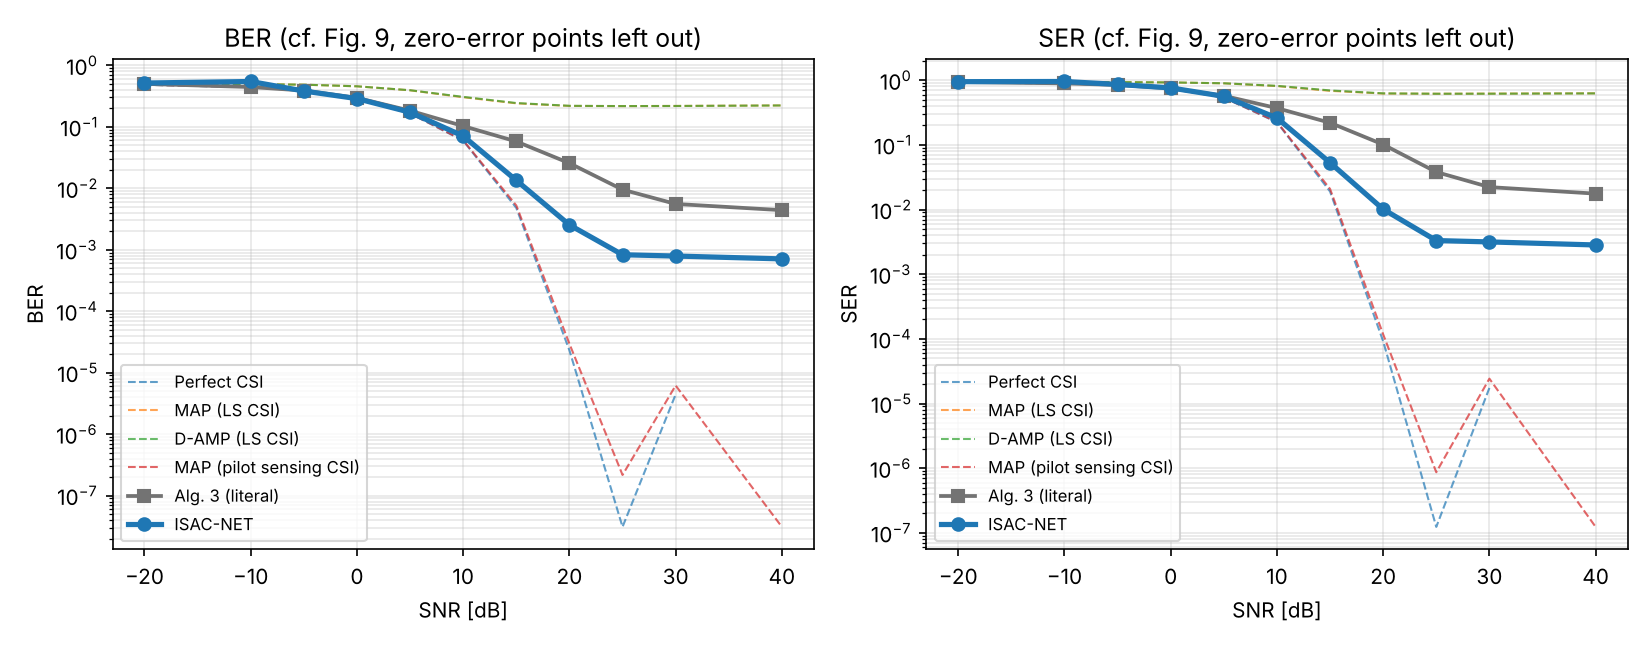
\includegraphics[width=\textwidth]{b_fig9.png}
\caption{BER (left) and SER (right) versus SNR. Thin dashed lines are baselines; points with zero errors are left out.}
\label{fig:ber}
\end{figure}

\begin{table}[H]
\centering\footnotesize
\setlength{\tabcolsep}{2.5pt}
\begin{tabular}{lccccccc}
\toprule
SNR (dB) & 0 & 5 & 10 & 15 & 20 & 25 & 30 \\
\midrule
Alg.~3, literal & \sci{3.0}{-1} & \sci{1.8}{-1} & \sci{1.0}{-1} & \sci{5.8}{-2} & \sci{2.6}{-2} & \sci{9.5}{-3} & \sci{5.6}{-3} \\
ISAC-NET (output, layer 5) & \sci{2.9}{-1} & \sci{1.7}{-1} & \sci{7.1}{-2} & \sci{1.3}{-2} & \sci{2.5}{-3} & \sci{8.3}{-4} & \sci{7.9}{-4} \\
ISAC-NET, layer 4 & \sci{2.9}{-1} & \sci{1.8}{-1} & \sci{8.3}{-2} & \sci{2.3}{-2} & \sci{1.7}{-3} & \sci{3.1}{-5} & \sci{2.8}{-6} \\
\bottomrule
\end{tabular}
\caption{Mean BER versus SNR.}
\label{tab:ber}
\end{table}

\begin{itemize}
  \item \textbf{Learning helps the literal algorithm.} ISAC-NET lowers BER by $4.3\times$ at 15 dB, $10\times$ at 20 dB, $11\times$ at 25 dB and $7\times$ at 30 dB compared with literal Alg.~3. This reproduces the paper's main claim. Below 5 dB there is little or no gain, as in~\cite{isacnet}.
  \item \textbf{The ``conventional'' receivers floor.} LS + MAP and D-AMP with the held LS estimate level off near BER 0.2, the shape of the paper's conventional curve.
  \item \textbf{The last layer limits high-SNR BER.} Output BER stays near \sci{8}{-4} from 25 to 40 dB, while layer 4 reaches \sci{3.1}{-5} at 25 dB and no errors at 40 dB. The fifth layer partly undoes the convergence of the earlier ones (Section~\ref{sec:layers}).
\end{itemize}

\subsection{Sensing (cf.\ Fig.~10 of~\texorpdfstring{\cite{isacnet}}{[1]})}\label{sec:sensing}
\begin{figure}[H]
\centering
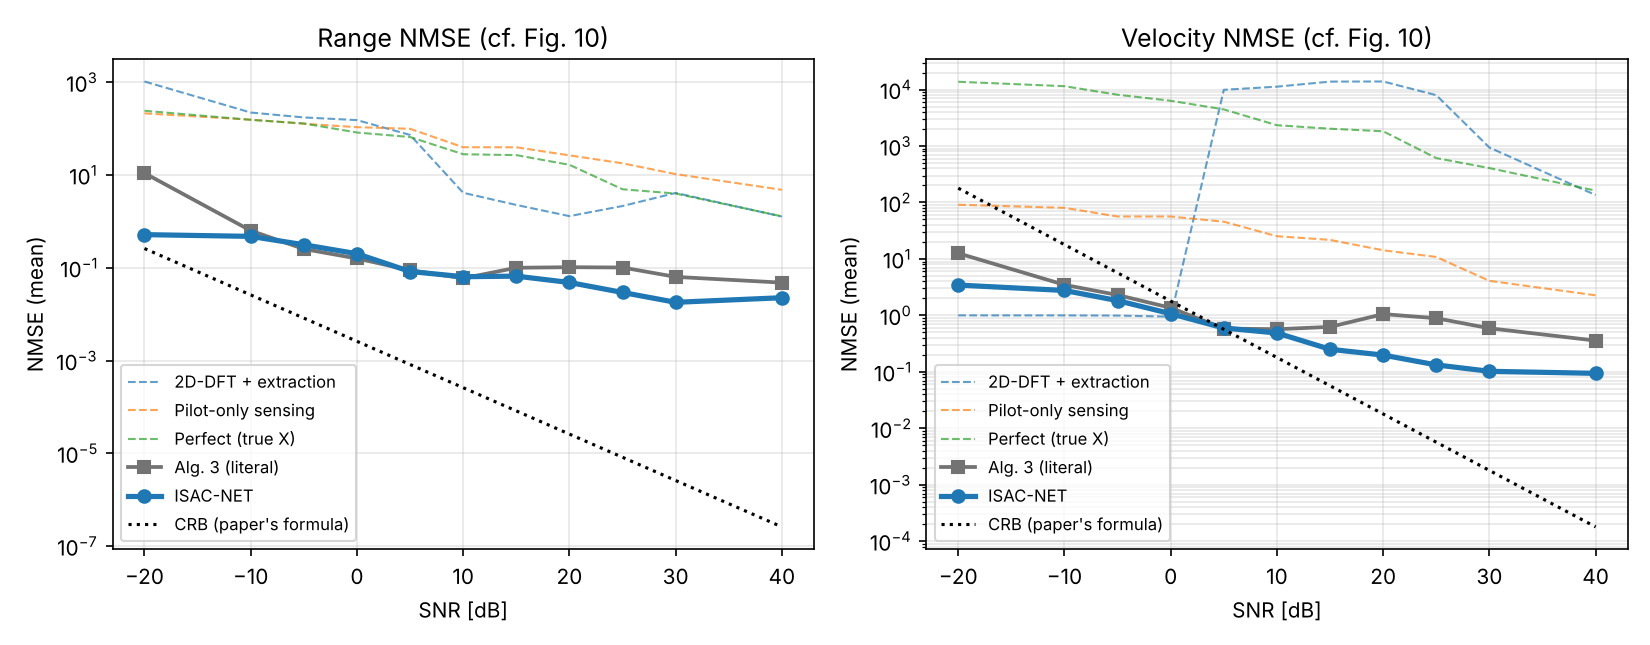
\includegraphics[width=\textwidth]{b_fig10.png}
\caption{Mean range (left) and velocity (right) NMSE versus SNR, with the CRB drawn from the paper's formula.}
\label{fig:nmse}
\end{figure}

ISAC-NET lowers the mean velocity NMSE from 1.05 to 0.20 at 20 dB and from 0.89 to 0.13 at 25 dB, and the mean range NMSE from 0.10 to 0.048 at 20 dB and to 0.029 at 25 dB. At 10 dB and below the two are about equal. Sensing from pilots alone, or by 2D-DFT on detected symbols without the joint loop, is one to three orders of magnitude worse. All methods stay well above the CRB, because the 28 m/s velocity bin is wider than the 5 m/s spacing of the targets; on-grid estimates cannot get much below velocity NMSE $10^{-2}$. Mean NMSE is driven by a few frames with a missed target: the median range NMSE is about $10^{-7}$ from 10 dB upwards for every receiver.

\subsection{Convergence over layers (cf.\ Fig.~8 of~\texorpdfstring{\cite{isacnet}}{[1]})}\label{sec:layers}
\begin{figure}[H]
\centering
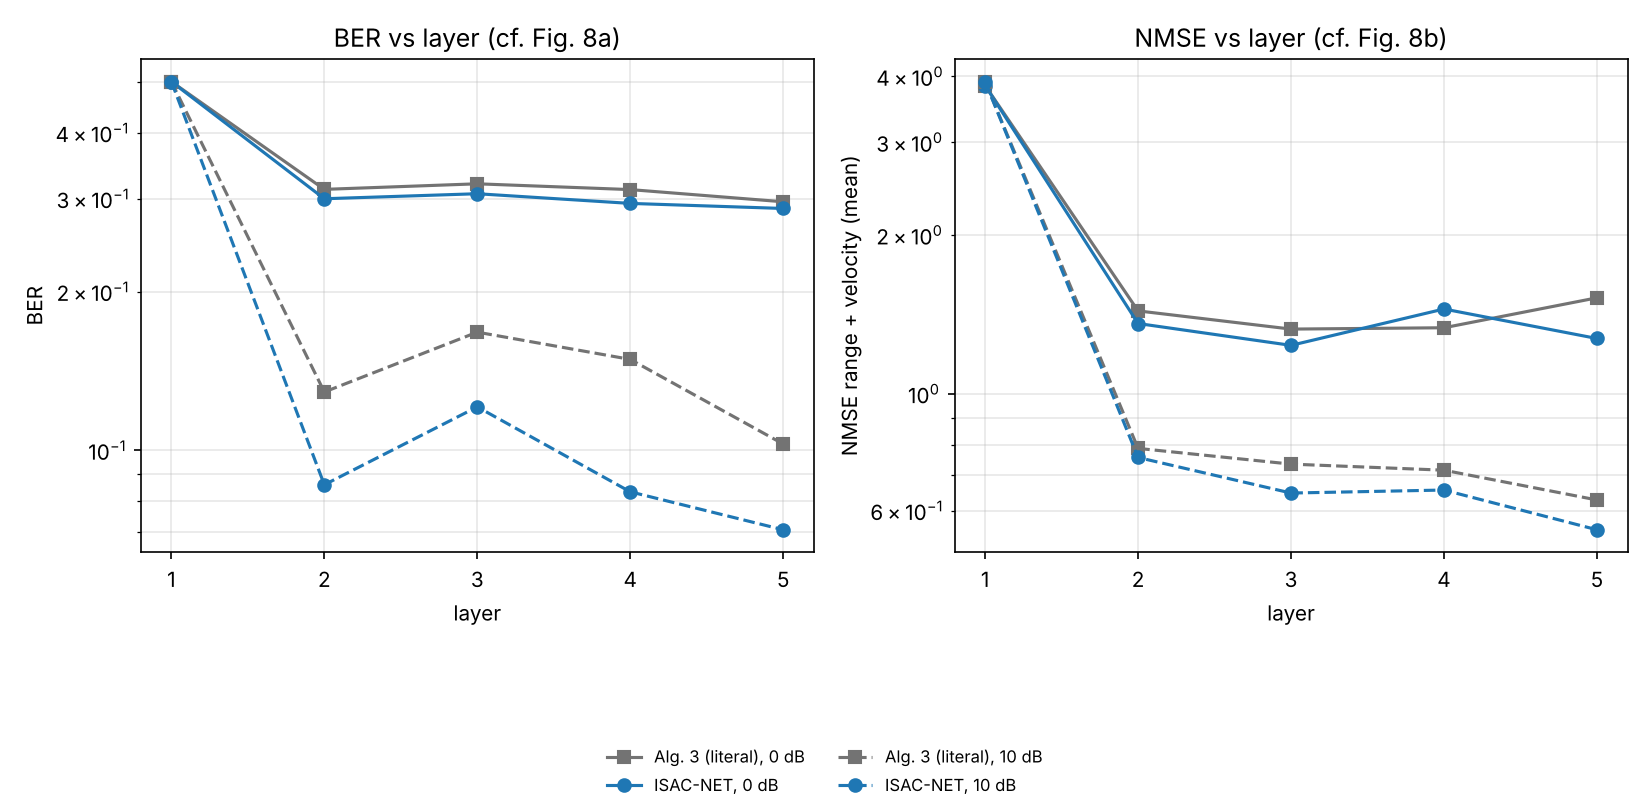
\includegraphics[width=\textwidth]{b_fig8.png}
\caption{BER (left) and range + velocity NMSE (right) after each layer, at 0 dB (solid) and 10 dB (dashed).}
\label{fig:layers}
\end{figure}

Literal Alg.~3 gets worse from layer 2 to layer 3 at every SNR above 0 dB (at 10 dB, BER 0.13 to 0.17), the oscillation noted in Table~\ref{tab:choices}. Learning does not remove it at layer 3, but it lowers every later layer: at 10 dB ISAC-NET ends at BER 0.071 against 0.10, and at 20 dB it reaches \sci{1.7}{-3} at layer 4 against \sci{2.6}{-2} for Alg.~3 at layer 5. At 0 dB all receivers are limited by noise and the layers change little.

\subsection{Comparison with the published figures}\label{sec:paper-comp}
Our curves have the same shape as the paper's: the conventional floor, the perfect-channel curve reaching $10^{-5}$ near 21 dB, and ISAC-NET lying between them and improving on the hand-set algorithm. Table~\ref{tab:diffs} lists the remaining differences and their causes.

\begin{table}[H]
\centering\small
\begin{tabularx}{\textwidth}{>{\raggedright\arraybackslash}p{3.6cm}>{\raggedright\arraybackslash}p{3.2cm}>{\raggedright\arraybackslash}X}
\toprule
Feature of~\cite{isacnet} & This work & Cause \\
\midrule
ISAC-NET close to the perfect channel & ISAC-NET levels off near \sci{8}{-4} & Fifth layer oscillation of the literal update (Table~\ref{tab:choices}); the paper may iterate D-AMP further than its text says \\
NMSE about $10^5$ below a threshold SNR & NMSE at most about 1 with the search window & Without the window, literal Alg.~3 has BER $\approx0.5$ and velocity NMSE $\approx4\times10^4$ at every SNR: a wrong far-off peak corrupts the rebuilt channel \\
Velocity NMSE down to $10^{-3}$--$10^{-4}$ & Best 0.094 & 28 m/s bin vs 5 m/s target spacing; needs off-grid estimation \\
CRB line almost flat & CRB falls $10\times$ per 10 dB & The drawn line does not follow the paper's own formula $\Delta R/\sqrt{2\,\mathrm{SNR}}$ \\
Fig.~8 uses 10 layers & 5 layers & A 10-layer training at learning rate 0.01 diverged \\
OAMP-Net2 and TPG curves & Not implemented & Out of scope \\
\bottomrule
\end{tabularx}
\caption{Remaining differences from the published figures.}
\label{tab:diffs}
\end{table}

\subsection{Unseen target layouts}\label{sec:unseen}
The network above was trained on the fixed targets of Table~\ref{tab:params}. To test how far it generalises, it was evaluated without retraining on random targets: path length 5--150 m (at least 5 m apart) and speed 3--30 m/s in either direction, drawn anew for every frame.

\begin{table}[H]
\centering\small
\begin{tabular}{lccccc}
\toprule
SNR (dB) & 10 & 15 & 20 & 25 & 30 \\
\midrule
Alg.~3, literal & \sci{1.1}{-1} & \sci{6.2}{-2} & \sci{3.5}{-2} & \sci{1.9}{-2} & \sci{1.5}{-2} \\
ISAC-NET (layer 5) & \sci{7.5}{-2} & \sci{2.2}{-2} & \sci{6.4}{-3} & \sci{4.4}{-3} & \sci{4.4}{-3} \\
\bottomrule
\end{tabular}
\caption{Mean BER on random target layouts never seen in training.}
\label{tab:unseen}
\end{table}

The gain falls from 4--11$\times$ to 3--5$\times$, and ISAC-NET levels off at \sci{4.4}{-3} instead of \sci{8}{-4}. The learned parameters are partly tuned to the training scenario.

\subsection{Extension: clutter in the channel}\label{sec:clutter}
The channel of~\cite{isacnet} contains only the target echoes. Real bistatic links also see clutter from buildings, ground and other static or slow objects. Following~\cite{clutter}, we add distributed clutter to the channel: $N_c$ scatterers per frame with path length uniform in 5--200 m, RCS log-uniform in $[0.01,1]\cdot\alpha_c\cdot\sigma_{\text{target}}$, and Doppler $f\sim\mathcal{N}(0,\sigma_{f,c}^2)$ with $\sigma_{f,c}=30$ Hz (about 2 m/s). Clutter is part of the true channel but is not a target, so it enters neither the sensing truth nor the loss. The trained ISAC-NET of Section~\ref{sec:comm}, which never saw clutter, is tested on 50 frames per point.

\begin{table}[H]
\centering\small
\begin{tabular}{lcccc}
\toprule
 & \multicolumn{2}{c}{20 dB} & \multicolumn{2}{c}{25 dB} \\
\cmidrule(lr){2-3}\cmidrule(lr){4-5}
Test clutter & Alg.~3 & ISAC-NET & Alg.~3 & ISAC-NET \\
\midrule
None & \sci{2.45}{-2} & \sci{2.35}{-3} & \sci{9.02}{-3} & \sci{6.46}{-4} \\
$N_c=5,\ \alpha_c=1$ & \sci{2.79}{-2} & \sci{4.40}{-3} & \sci{1.50}{-2} & \sci{1.76}{-3} \\
$N_c=20,\ \alpha_c=0.1$ & \sci{2.77}{-2} & \sci{4.18}{-3} & \sci{1.55}{-2} & \sci{3.74}{-3} \\
$N_c=20,\ \alpha_c=1$ & \sci{3.14}{-2} & \sci{6.59}{-3} & \sci{1.96}{-2} & \sci{6.58}{-3} \\
\bottomrule
\end{tabular}
\caption{Mean BER under clutter (literal Alg.~3 and ISAC-NET, 5 layers, 50 frames per point).}
\label{tab:clutter}
\end{table}

\begin{itemize}
  \item \textbf{Communication is robust to clutter.} ISAC-NET keeps a 3--6$\times$ BER gain over Alg.~3 in every condition. Heavy clutter sets a BER floor near \sci{6}{-3} above 20 dB, because the channel is rebuilt from the $L_p$ target paths only and the unmodelled clutter becomes residual interference.
  \item \textbf{Sensing is not.} With even 5 scatterers, mean range NMSE at 25 dB rises from 0.014 to about 0.2--0.3 and velocity NMSE to 0.4--0.7 for both receivers: the cyclic peak extraction reports clutter peaks as targets.
  \item \textbf{Retraining the step sizes is not enough.} Retraining $\Omega$ on frames with random clutter lowers BER under clutter by only 15--25\% and leaves the sensing NMSE unchanged. The clutter Doppler ($\approx2$ m/s) is far below one velocity bin ($\approx14$ m/s), so no choice of step sizes or threshold can separate clutter from slow targets; the receiver needs a new processing stage.
\end{itemize}

% =====================================================================
\section{Future Work: Clutter-Robust ISAC-NET}\label{sec:future}
The direction for the next semester is to make ISAC-NET work in a cluttered channel, since Section~\ref{sec:clutter} shows that clutter, which the paper does not model, breaks its sensing chain while leaving communication largely intact.

\paragraph{Problem.} ISAC-NET reconstructs the channel from a few point targets and senses them by picking peaks in the range--Doppler map. Clutter adds many weak, slow scatterers. They become false targets in sensing, and, because the rebuilt channel leaves them out, residual interference in detection. The learnable step sizes of ISAC-NET cannot remove either effect.

\paragraph{Proposed approach.}
\begin{enumerate}
  \item \textbf{Learned clutter suppression before sensing.} Insert a clutter-removal stage on the range--Doppler map, for example the residual/attention U-Net of~\cite{clutter}, inside each ISAC-NET layer, and train it jointly with the step sizes so that detection and sensing errors both shape it.
  \item \textbf{Clutter-aware channel reconstruction.} Add a low-Doppler clutter term to the rebuilt channel, estimated from the residual, so that clutter is cancelled in detection instead of acting as interference. This targets the BER floor of Table~\ref{tab:clutter}.
  \item \textbf{One model for all conditions.} Train on frames with random SNR, clutter density, clutter power and target layouts, so that one trained network serves every operating point and generalises to unseen target positions (Section~\ref{sec:unseen}).
  \item \textbf{Evaluation.} Report detection and false-alarm probability as well as range/velocity NMSE and BER, against clutter density and clutter-to-noise ratio, and compare with a classical zero-Doppler notch and with~\cite{clutter}.
\end{enumerate}

\paragraph{Other gaps.} Table~\ref{tab:gaps} lists further issues found during the reproduction, which can be studied alongside.

\begin{table}[H]
\centering\small
\begin{tabularx}{\textwidth}{>{\raggedright\arraybackslash}p{3.6cm}>{\raggedright\arraybackslash}X>{\raggedright\arraybackslash}p{4.2cm}}
\toprule
Gap & Evidence & Possible work \\
\midrule
Generalisation to other target layouts & Learning gain falls from 4--11$\times$ to 3--5$\times$ on unseen layouts (Section~\ref{sec:unseen}) & Training over random placements and target counts \\
Closely spaced targets & 5 m/s target spacing is below the 28 m/s velocity bin & Off-grid or super-resolution estimation \\
Last-layer oscillation & Layer 4 beats layer 5 by $25\times$ at 25 dB & Loss on every layer's output (deep supervision) \\
Complexity claim & $\BH_\varphi$ is diagonal, so a layer costs $O(L_pN_tN_rMN)$, not $O(L_pN_tN_r(MN)^2)$ & Corrected analysis \\
\bottomrule
\end{tabularx}
\caption{Further gaps found during the reproduction.}
\label{tab:gaps}
\end{table}

% =====================================================================
\section{Conclusion}\label{sec:conclusion}
This project reproduced ISAC-NET at full size under the paper's simulation setup and confirmed its main claim: learning the step sizes of the literal one-update algorithm lowers BER by 4--11$\times$ at 15--25 dB and velocity NMSE by about 5$\times$ at 20 dB. The reproduction also explained the remaining differences from the published figures, chiefly unstated details such as the SNR definition, the LS reference and the sensing search range.

Two qualifications emerged. The learned parameters transfer only partly to target layouts not seen in training, and the last unfolded layer partly undoes the convergence of the earlier ones.

Adding clutter to the channel showed that ISAC-NET's communication is robust but its sensing is not, and that retraining its step sizes cannot fix this. Next semester's work is therefore a clutter-robust ISAC-NET: a learned clutter-suppression stage before sensing and a clutter-aware channel reconstruction, trained jointly as one model for all SNR and clutter conditions. The code, results and figures are at \url{https://github.com/Kushal2oo4/isac-net}.

% =====================================================================
\begin{thebibliography}{9}
\bibitem{isacnet} W.~Jiang, D.~Ma, Z.~Wei, Z.~Feng, P.~Zhang and J.~Peng, ``ISAC-NET: Model-driven deep learning for integrated passive sensing and communication,'' \emph{IEEE Trans.\ Commun.}, vol.~72, no.~8, pp.~4692--4707, Aug.~2024, doi: 10.1109/TCOMM.2024.3375818.
\bibitem{zhang2022} J.~A. Zhang \emph{et al.}, ``Enabling joint communication and radar sensing in mobile networks---A survey,'' \emph{IEEE Commun.\ Surveys Tuts.}, vol.~24, no.~1, pp.~306--345, 2022.
\bibitem{oampnet} H.~He, C.~Wen, S.~Jin and G.~Y. Li, ``Model-driven deep learning for MIMO detection,'' \emph{IEEE Trans.\ Signal Process.}, vol.~68, pp.~1702--1715, 2020.
\bibitem{sturm2011} C.~Sturm and W.~Wiesbeck, ``Waveform design and signal processing aspects for fusion of wireless communications and radar sensing,'' \emph{Proc.\ IEEE}, vol.~99, no.~7, pp.~1236--1259, Jul.~2011.
\bibitem{clutter} Y.~E. Sagduyu, T.~Erpek and S.~Kompella, ``Multistatic ISAC with deep learning-based clutter suppression for 5G and beyond,'' arXiv:2610.40586, Oct.~2026.
\end{thebibliography}

% =====================================================================
\appendix
\section{Code and Reproducibility}
{\sloppy The repository \url{https://github.com/Kushal2oo4/isac-net} contains the simulator (\texttt{isacnet/}), the scripts for every result in this report (\texttt{scripts/}), the result files and figures (\texttt{results/}) and unit tests (\texttt{tests/}). Each figure is regenerated by one script:\par}

\begin{table}[H]
\centering\small
\begin{tabular}{ll}
\toprule
Result & Script \\
\midrule
Baselines & \texttt{scripts/sweep\_baselines.py} \\
Training (Table~\ref{tab:train}) & \texttt{scripts/train\_isacnet.py --joint --lr 0.002} \\
Evaluation, Tables~\ref{tab:ber}--\ref{tab:unseen} & \texttt{scripts/eval\_isacnet.py} \\
Unseen targets, Table~\ref{tab:unseen} & \texttt{scripts/eval\_isacnet.py --random-targets} \\
Figs.~\ref{fig:ber}--\ref{fig:layers} & \texttt{scripts/plot\_final.py} \\
Clutter, Section~\ref{sec:clutter} & \texttt{scripts/run\_clutter\_train.sh}, \texttt{scripts/run\_clutter\_check.sh} \\
\bottomrule
\end{tabular}
\caption{Scripts that regenerate each result.}
\end{table}

\end{document}
